%##############################################################################
%## COPYRIGHT NOTICE ##########################################################
% Produced by dendrogram.py .
% Copyright (C) 2016-2017 Juan I. Perotti
%
% This program/code is free software; you can redistribute it and/or modify
% it under the terms of the GNU General Public License as published by
% the Free Software Foundation; either version 2 of the License, or
% (at your option) any later version.
%
% This program is distributed in the hope that it will be useful,
% but WITHOUT ANY WARRANTY; without even the implied warranty of
% MERCHANTABILITY or FITNESS FOR A PARTICULAR PURPOSE.  See the
% GNU General Public License for more details.
%
% You should have received a copy of the GNU General Public License
% along with this program; if not, write to the Free Software
% Foundation, Inc., 59 Temple Place, Suite 330, Boston, MA  02111-1307  USA
% 
% See http:#www.gnu.org/licenses/gpl.txt for more details.
% 
%##############################################################################
% Author       : Juan Ignacio Perotti ( juanignacio.perotti@imtlucca.it )
% Collaborators: Claudio Juan Tessone, Aaron Clausset and Guido Caldarelli
% Project      : Generalized Hierarchical Random Graphs
% Location     : Institute for Advanced Studies Lucca, Piazza S.Francesco, 19, 
%                55100 Lucca LU, Italy.
% Created      : 1 March 2016
% Modified     : -- (cleaned up for public consumption)
% 
%##############################################################################

% The standalone documentclas fit the page of the pdf to the size of the 
% content.
\documentclass{standalone}

\usepackage[obeyspaces]{url}
\usepackage{tikz}
\usetikzlibrary{shapes}

% If we like to control the size of the page...
%\usepackage[paperwidth=17cm,paperheight=21cm,hmargin=0cm,vmargin=0cm]{geometry}

% To impede the edges overlap with the nodes.
\pgfdeclarelayer{bg}    % declare background layer
\pgfsetlayers{bg,main}  % set the order of the layers (main is the standard layer)

% Define a more convenient macro without @ in its name
\def\gprgb#1#2#3{rgb,255:red,#1;green,#2;blue,#3}

\begin{document}

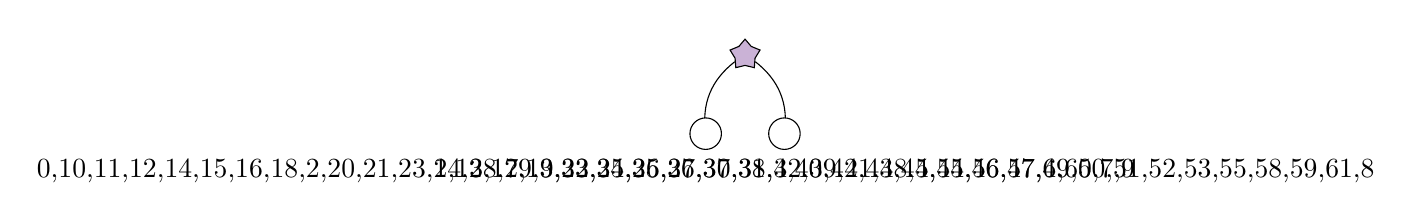
\begin{tikzpicture}

% Put legends if any...


% Draw the nodes...
\node (2) at (    0.5000,    1.0000) [shape=star, star points=5,fill=\gprgb{202}{178}{214},inner sep=1pt,minimum size=4mm,draw,label=above right:] {};
\node (0) at (    0.0000,    0.0000) [shape=circle,fill=white,inner sep=1pt,minimum size=4mm,draw,label=below:{0,10,11,12,14,15,16,18,2,20,21,23,24,28,29,3,33,34,35,36,37,38,4,40,42,43,44,45,46,47,49,50,51,52,53,55,58,59,61,8}] {};
\node (1) at (    1.0000,    0.0000) [shape=circle,fill=white,inner sep=1pt,minimum size=4mm,draw,label=below:{1,13,17,19,22,25,26,27,30,31,32,39,41,48,5,54,56,57,6,60,7,9}] {};


% Draw the edges...
\begin{pgfonlayer}{bg}
\draw (2) edge[bend right,color=black!100] (0.center);
\draw (2) edge[bend left,color=black!100] (1.center);

\end{pgfonlayer}

\end{tikzpicture}

\end{document}
